\begin{frame}
    \frametitle{Containerization under the hood}
    \framesubtitle{Bare Metal}
    \centering 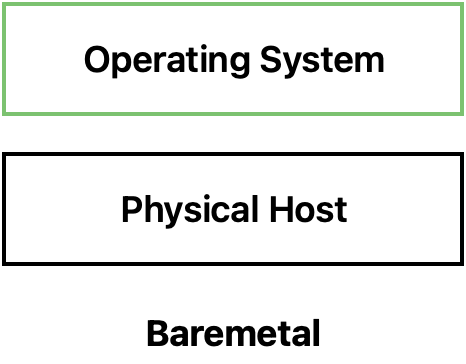
\includegraphics[width=0.5\textwidth]{images/baremetal}
\end{frame}

\begin{frame}
    \frametitle{Containerization under the hood}
    \framesubtitle{Hypervisors}
    \centering 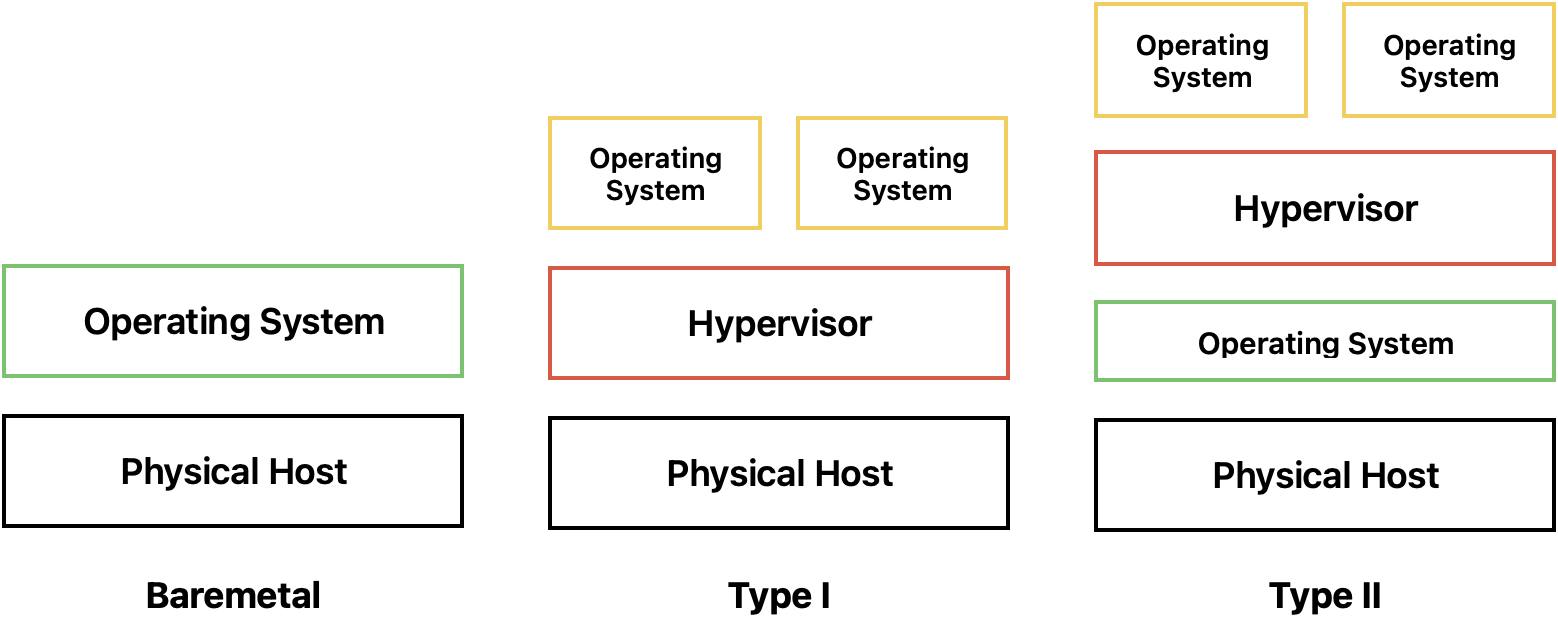
\includegraphics[width=\textwidth]{images/baremetal_vs_hv}
\end{frame}

\begin{frame}
    \frametitle{Containerization under the hood}
    \framesubtitle{Containers I}
    \centering 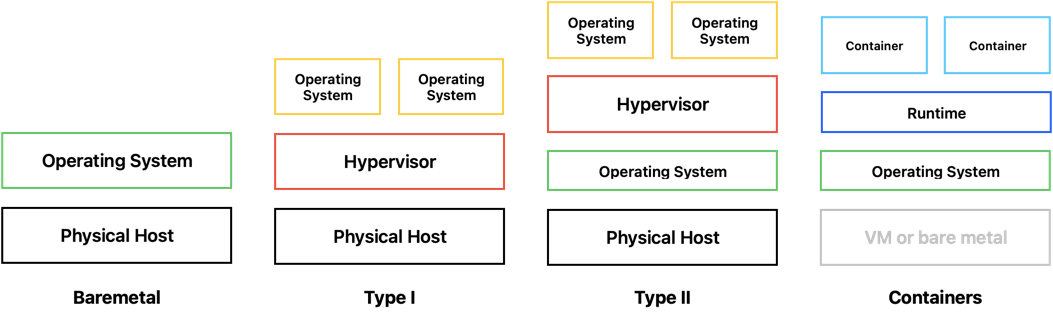
\includegraphics[width=\textwidth]{images/containers}
\end{frame}

\begin{frame}
    \frametitle{Containerization under the hood}
    \framesubtitle{Containers II}
    \begin{itemize}
        \item Containers are isolated processes
        \item No need for virtualized hardware
    \end{itemize}
    \vspace{0.5cm}
    You can see this quite obviously with the commands on the following slide.
\end{frame}

\begin{frame}[fragile]
    \frametitle{Containerization under the hood}
    \framesubtitle{Containers III}
    On a Linux system hosting VMs run:
    \vspace{0.5cm}
    \begin{lstlisting}[language=bash]
ps aux | grep kvm
    \end{lstlisting}
    \vspace{0.5cm}
    On a Linux machine with docker installed run:
    \vspace{0.5cm}
    \begin{lstlisting}[language=bash]
docker run -dit --name alpine alpine:latest /bin/ash
    \end{lstlisting}
    \begin{lstlisting}[language=bash]
ps -fp $(docker inspect -f '{{.State.Pid}}' alpine)
    \end{lstlisting}
\end{frame}

\begin{frame}[fragile]
    \frametitle{Containerization under the hood}
    \framesubtitle{Containers IV}
    The container likely only runs one single process.\\
    This process likely hast the ID \texttt{1}.
    \vspace{0.5cm}
    \begin{lstlisting}[language=bash]
docker exec -it alpine ps aux
    \end{lstlisting}
\end{frame}

\begin{frame}[fragile]
    \frametitle{Containerization under the hood}
    \framesubtitle{\texttt{rootfs} I}
    Notice we started the container with \texttt{/bin/ash}.\\
    This does not ship standard with most distributions.\\
    So where does this binary come from?
    \vspace{0.5cm}
    \begin{lstlisting}[language=bash]
ROOT_FS=$(docker inspect \
    $(docker ps -q --filter "name=alpine") \
    | jq '.[0].GraphDriver.Data.MergedDir' \
    | sed 's/"//g' \
)
    \end{lstlisting}
\end{frame}

\begin{frame}[fragile]
    \frametitle{Containerization under the hood}
    \framesubtitle{\texttt{rootfs} II}
    We now have the path to the containers filesystem saved in the variable \texttt{Root\_FS}.\\
    We can now search if the \texttt{ash} binary is present.
    \vspace{0.5cm}
    \begin{lstlisting}[language=bash]
sudo ls $ROOT_FS/bin | grep ash
    \end{lstlisting}
\end{frame}

\begin{frame}
    \frametitle{Containerization under the hood}
    \framesubtitle{Namespaces I}
    \begin{itemize}
        \item Namespaces are borders in which a process can operate.
        \item They isolate processes and therefore containers from another.
        \item We can check the namespaces of a process under the \texttt{/proc} directory.
    \end{itemize}
\end{frame}

\begin{frame}[fragile]
    \frametitle{Containerization under the hood}
    \framesubtitle{Namespaces II}
    The following command shows us the namespaces of our Alpine container.
    \vspace{0.5cm}
    \begin{lstlisting}[language=bash]
ls -l /proc/$(docker inspect \
    --format '{{.State.Pid}}' alpine)/ns
    \end{lstlisting}
\end{frame}

\begin{frame}
    \frametitle{Containerization under the hood}
    \framesubtitle{Namespaces III}
    \begin{itemize}
        \item Processes can have the same ID as long as they are in different namespaces.
        \item This is why the process ID of the container process is \texttt{1}.
        \item The host system most likely runs \texttt{/sbin/init} with process ID \texttt{1}.
    \end{itemize}
\end{frame}

\begin{frame}
    \frametitle{Containerization under the hood}
    \framesubtitle{Control Groups I}
    \begin{itemize}
        \item Cgroups are a way to limit resources of a process.
        \item They are used to limit CPU, memory, and other resources.
        \item We can check the cgroups of a process under the \texttt{/proc} directory.
    \end{itemize}
\end{frame}

\begin{frame}[fragile]
    \frametitle{Containerization under the hood}
    \framesubtitle{Control Groups II}
    Check the cgroups of our Alpine container.
    \vspace{0.5cm}
    \begin{lstlisting}[language=bash]
sudo cat /proc/$(docker inspect \
    --format '{{.State.Pid}}' alpine)/cgroup
    \end{lstlisting}
    \vspace{0.5cm}
    \texttt{0::/system.slice/docker-xxx.scope}
\end{frame}

\begin{frame}
    \frametitle{Containerization under the hood}
    \framesubtitle{Control Groups III}
    \begin{itemize}
        \item \texttt{0::}\\
        Root \texttt{cgroup}
        \item \texttt{system.slice}\\
        Broadly speaking this handles processes started by \texttt{systemd}
        \item \texttt{docker-589c53b502....scope}\\
        The container specific \texttt{cgroup}
    \end{itemize}
    \vspace{0.5cm}
    The hierarchy allows the host system to control resources of service.\\
    Systemd can control the resources of all services started by it.\\
    Docker can control the resources of all containers started by it.
\end{frame}
